\documentclass[11pt,a4paper, twoside]{article}
\usepackage[top=2.5cm, bottom=2.5cm, left=3.5cm, right=2.5cm]{geometry}
\usepackage{setspace}
\setstretch{1.25}
\usepackage{polski}
\usepackage[utf8]{inputenc}
\usepackage{graphicx}
\usepackage{pdfpages}
\usepackage{minted}
\usemintedstyle{trac}
\usepackage{helvet}
% \renewcommand{\familydefault}{\sfdefault}
\usepackage{sectsty}
% \sectionfont{\rmfamily}
\usepackage{indentfirst}
\usepackage{hyperref}
\usepackage{subcaption}
\usepackage{graphicx}
\setlength{\footskip}{40pt}
\setcounter{secnumdepth}{5}
\makeatletter
\renewcommand\subparagraph{\@startsection{paragraph}{6}{\z@} %
	{-3.25ex\@plus -1ex \@minus -.2ex} %
	{0.0001pt \@plus -1ex \@minus -.2ex} %
	{\normalfont\normalsize}}
\makeatother
\usepackage{chngcntr}
\usepackage{float}
\counterwithin{subfigure}{figure}
\begin{document} 

\includepdf[pages={1,2}]{first-pages.pdf}
\tableofcontents

%\begin{minipage}{\linewidth}
\newpage
\cleardoublepage
\section{Cel i zakres pracy}
Przedmiotem niniejszej pracy jest budowa mobilnego systemu pomiaru czasu dla zawodów narciarskich. System składa się z dwóch bramek: startowej oraz końcowej, które wykorzystują wiązke laserową w celu uchwycenia dokładnego momentu przejechania zawodnika przez bramkę. 

Niniejsza praca będzie się składać z trzech głównych części. Pierwsza z nich poświęcona zostanie architekturze systemu i wykorzystanych technologiach, a w szczególności, komunikacji pomiędzy komponentami oraz podstawą teoretycznym działania. Druga część tej pracy zawiera opis implementacji, zaś trzecia część jest poświęcona umieszczeniu systemu w obudowie ochronnej.
\section{Wstęp}
Obecnie na rynku istnieją podobne systemy do tego, którego budowę ta praca przedstawia, jednak często kosztują tysiące złotych. Praca ta jest próbą stowrzenia rozwiązania spełniającego podobne zadanie do ww. systemów korzystając z ogólnie dostępnych podzespołów.

Jako szkielet systemu zostało wybrane Raspberry Pi - platforma komputerowa stworzona przez Raspberry Fundation. W momencie premiery (29 luty 2012) model B użyty w tej pracy miał cenę początkową US\$ 35. Raspberry Pi oparte jest o chip BCM2835 zawierający procesor ARMv6. Urządzenie działa pod kontrolą dystrybucji systemu Linux Raspbian będącą portem Debiana Wheezy koniecznym z powodu braku kompatybilności (oficjalne wydanie Debiana Wheezy na platformę armhf działa jedynie z procesorami ARMv7 lub nowszymi).

Obie aplikacjie (startowa i końcowa) zostały napistane przy użyciu języka Ruby 2.1.0 oraz dla aplikacji startowej stworzony został interface web umożliwiający wprowadzanie zawodników oraz podgląd wyników, jak również import oraz eksport. Napisany został on przy użyciu CoffeeScript oraz biblioteki JavaScript Backbone.js. 
CoffeeScript jest językiem inspirowanym elegancką składnią Ruby i Pythona, który kompiluje się do JavaScriptu. Backbone.js natomiast zapewnia strukturę aplikacji.
%\newline
%W momencie pisania kodu aplikacji autor nie zdawał sobie jeszcze sprawy z pewnych dobrych pratyk pisania kodu JavaScript, zatem w kodzie znajdują się błędy, których należy unikać. Z tego powodu ta praca będzie się też starać je pokazać, na czym one polegają i jakie trudności w późniejszym utrzymaniu kodu podowują tak aby czytelnik był ich świadom i sam ich nie popełniał.
\newline
\newline
\noindent
W pracy zostały użyte różne \emph{gemy}~-~programy i biblioteki managera paczek \emph{RubyGems}, których lista w raz z licencjami zostanie przedstawiona na końcu tej pracy.
\newline

\noindent
Kompletny kod źródłowy pracy można znaleźć pod adresami:
\newline
\url{https://github.com/okapusta/skirace}
\newline
\url{https://github.com/okapusta/skirace-worker}

\newpage

%\end{minipage}
\newpage
\noindent
\section{Realizacja tematu}
\subsection{Architektura}
System którego ta praca dotyczy został zbudowany w myśl modelu master/slave gdzie masterem jest aplikacja początkowa. To tam znajduje się interface, baza danych oraz serwer Memcached. W momencie uruchomienia aplikacji, oprócz startu serwera serwującego aplikację WEB tworzony jest nowy wątek zawierający event loop, który rejestruje przecięcie wiązki lasera, a kiedy to sie stanie, ustawia godzinę tego zdarzenia w bazie danych.

Zadaniem workera jest zarejestrowanie przecięcia limii mety a kiedy to sie sanie worker wysyła rządanie POST do aplikacji startowej, która w podpwiedzi zwraca obliczony końcowy czas oraz imie i nazwisko zawodnika wyświetlane na LCD.
\newline

\begin{figure}[ht]
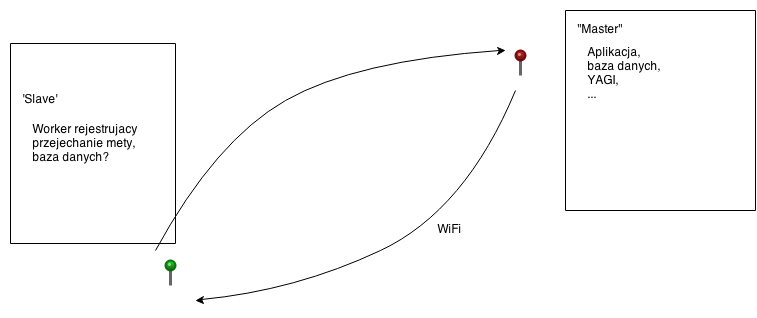
\includegraphics[scale=0.5]{./img/asdasd.png}
\caption{Architektura systemu}
\end{figure}
\noindent
Komunikacjia pomiędzy dwiema bramkami odbywa się poprzez WiFi.
\subsection{Wybrane technologie}
\subsubsection{Memcached}
Memcached jest to rozproszony system buforowania pamięci podręczniej oryginalnie zaprojektowany na potrzeby serwisu  LiveJournal. Pozwala on na przechowywanie obiektów w pamięci RAM przy pomocy kluczy \mbox{(key-value store)}. W aplikacji wykorzystany został w celu przechowania id aktualnego wyścigu.
\subsubsection{Dependency Injection}
W ninejszej pracy został wykorzystany wzorzec projektowy \emph{Dependency Injection (DI)} polegający na usuwaniu bespośrednich zależności klas na rzecz \emph{wstrzykiwania} ich w czasie konstruowania obiektu. Do osiągnięcia tego celu i uproszczenia  DI użyty został gem Dependor, udostępniający zestaw metod i modułów przeznaczony do tego celu.

Poniżej zamieszczone są listingi przedstawiające normlne wstrzykiwanie zależności w Ruby oraz z wykorzystaniem gemu Dependor.
\newline


\begin{figure}[H]
\centering
\begin{subfigure}[t]{0.45\textwidth}
\caption{Ruby}
\begin{listing}[H]
\inputminted[linenos=true]{ruby}{./src/di_ruby.rb}
\end{listing}
\end{subfigure}
\begin{subfigure}[t]{0.45\textwidth}
\caption{Ruby + Dependor}
\begin{listing}[H]
\inputminted{ruby}{./src/di_dependor.rb}
\end{listing}
\end{subfigure}
\end{figure}
\subsubsection{Sprockets}
Do kompilacji CoffeeScript oraz szablonów \emph{.hamlc} (\emph{Haml Coffee Assets}) został użyty gem \emph{Sprockets} zawierający preprocessory dla języków takich jak CoffeeScript czy SCSS. Sprockets w środowisku developerskim pozwala na kompilacje assetów (JavaScriptów i CSSów) 'w locie', natomiast w środowisku produkcyjnym assety są prekompilowane. Sprockets pozwala również na minifikacje zasobów to jest zastąpienie nazw funkcji czy zmiennych pojedyńczymi znakami w celu zmiejszenia rozmiaru kodu, który musi zostać pobrany przez przeglądarkę. 

Sprockets działa w kontekście Rack - minimalnego interfejsu dla aplikacji Ruby do komunikacji z popularnymi serwerami WWW. Zasoby serwowane przez sprockets są montowane w pliku \emph{config.ru}, będącym plikiem konfiguracyjnym dla interfejsu Rack poprzez który aplikacja jest uruchamiana. To tutaj tworzony jest wątek rejestrujący przejechanie linii startu oraz tutaj montowana jest ścieżka serwera WWW '/' tak aby pokazywała na aplikację Sinatra. 
\noindent
Samo sprockets jest montowane w następujący sposób:
\begin{listing}[H]
\inputminted[linenos=true]{ruby}{./src/sprockets_mount.rb}
\caption{config.ru}
\end{listing}
\noindent
Wykorzystane tutaj zmienne klasowe (\emph{assets\_prefix}, \emph{sprockets}) aplikacji są definiowane w pliku \emph{application.rb} zawierającym klasę aplikacji Sinatra.
\begin{listing}[H]
\inputminted[linenos=true]{ruby}{./src/sprockets_config.rb}
\caption{Ustawienie zmiennych Sprockets}
\end{listing}
\noindent
\begin{listing}[H]
\inputminted[linenos=true]{ruby}{./src/sprockets_asset_paths.rb}
\caption{Przeszukiwane foldery}
\end{listing}
\noindent
Powyższe listingi umieszczają skompilowane pliki z wyznaczonych ścieżek w folderze \emph{public/assets} pod nazwami \emph{application.js} oraz \emph{application.css}. Pliki te zawierają jedynie assety załączone poleceniem \emph{require} w plikach app/assets/javascripts/application.js i \newline app/assets/stylesheets/application.css.
\begin{listing}[H]
\inputminted[linenos=true]{javascript}{./src/application.js}
\caption{app/assets/javascripts/application.js}
$\label{aplication-js}$
\end{listing}
\begin{listing}[H]
\inputminted[linenos=true]{javascript}{./src/application.css}
\caption{app/assets/stylesheets/application.css}
\end{listing}
\subsubsection{Twitter Bootstrap}
Twitter Bootstrap jest frameworkiem front-end dostarczającym style CSS oraz kod JavaScript, który za zadanie ma przyśpieszenie budowę front-endu aplikacji. Bootstrap dostarcza zestaw klas HTML, które posiadają określone style. W tej pracy wykorzystany został Twitter Bootstrap w wersji drugiej. Aktualna wersja Bootstrapa to 3.1.1.
\subsubsection{HAML}
W projekcie został użyty HAML (HTML Abstraction Markup Language), który sprawia że kod jest przyjemniejszy do pisania i czytania. W HAML używa się jedynie tagów otwierających a o tym jak osadzone są elementy decyduje indentacja. HAML posiada też skróty na sekcje div o podanym id lub klasie.
\begin{figure}[H]
\centering
\begin{subfigure}[t]{0.45\textwidth}
\caption{HAML}
\begin{listing}[H]
\inputminted[linenos=true]{haml}{./src/example.haml}
\end{listing}
\end{subfigure}
\begin{subfigure}[t]{0.45\textwidth}
\caption{HTML}
\begin{listing}[H]
\inputminted{html}{./src/example.html}
\end{listing}
\end{subfigure}
\end{figure}
$\label{haml}$
Powyższe listingi przedstawiają przykładowy kod HAML oraz HTML do którego on się kompiluje.
\subsubsection{Backbone.js}
Backbone.js jest lekką biblioteką JavaScript nadającą strukturę aplikacją JavaScript. Typowe użycie tej biblioteki jest to zazwyczaj trio pomiędzy samym backbonem a jQuery i underscore.js.

W tej pracy został też użyty gem haml\_coffee\_assets pozwalający na pisanie szablonów Backbone w języku HAML z osadzonym CoffeeScriptem (podobnie jak w eRuby). 

Biblioteka Backbone.js stara się odtworzyć to co jest po stronie serwera w modelu MVC na stronę klienta (przeglądarki) i JavaScriptu. Model odzwierciedla zasób na serwerze i jest odpowiednikiem modelu po stronie serwera. Kolekcja jest grupą modeli pobieraną z serwera. Na kolekcji zdefiniowane są zdarzenia (eng. \emph{events}), które ponownie renderują widok np. kiedy element zostanie dodany do kolekcji. W Backbone Router odpowiedzialny jest za tłumaczenie adresów URL na widoki oraz za obsługę historii przeglądarki. Widok jest odpowiednikiem kontrolera znanego z Rails. Odpowiada na zdarzenia w oknie przeglądarki takie jak kliknięcie myszką i podejmuje odpowiednie akcje. Szablony natomiast są, w przypadku tej pracy, kodem HAML używanym przez widoki do renderowania treści aplikacji.
\subsection{Komunikacja}
Oba urządzenia komunikują się ze sobą przy pomocy WiFi w trybie pracy Ad Hoc. Jako karta sieciowa została wybrana karta USB TP-Link \mbox{TL-WN722N} ponieważ posiada antenę o zysku 4dBi, którą można odkręcić oraz zamontować mocniejszą antenę. Poniższy listing przedstawia konfiguracje urządzenia do pracy w trybie Ad Hoc.
\begin{listing}[H]
\inputminted[linenos=true]{sh}{./src/adhoc}
\caption{/etc/network/interfaces}
\end{listing}
Plik \emph{/etc/network/interfaces} drugiego urządzenia został skonfigurowany analogicznie. Różni sie on jedynie adresem IP ustawionym na \emph{192.168.10.2}. Urządzenia ustawione w trybie pracy Ad Hoc wykrywają się nawzajem i tworzą sieć o SSID SKIRACE.
\newpage
\subsection{Podstawy działania}
Ten rozdział ma na celu przedstawienie budowy oraz podstaw teoretycznych działania czujnika rejestrującego przecięcie wiązki lasera. Składa sie on z fotorezystora, rezystora oraz kondensatora. Poniższy rysunek przedstawia jego budowę.
\begin{figure}[h]
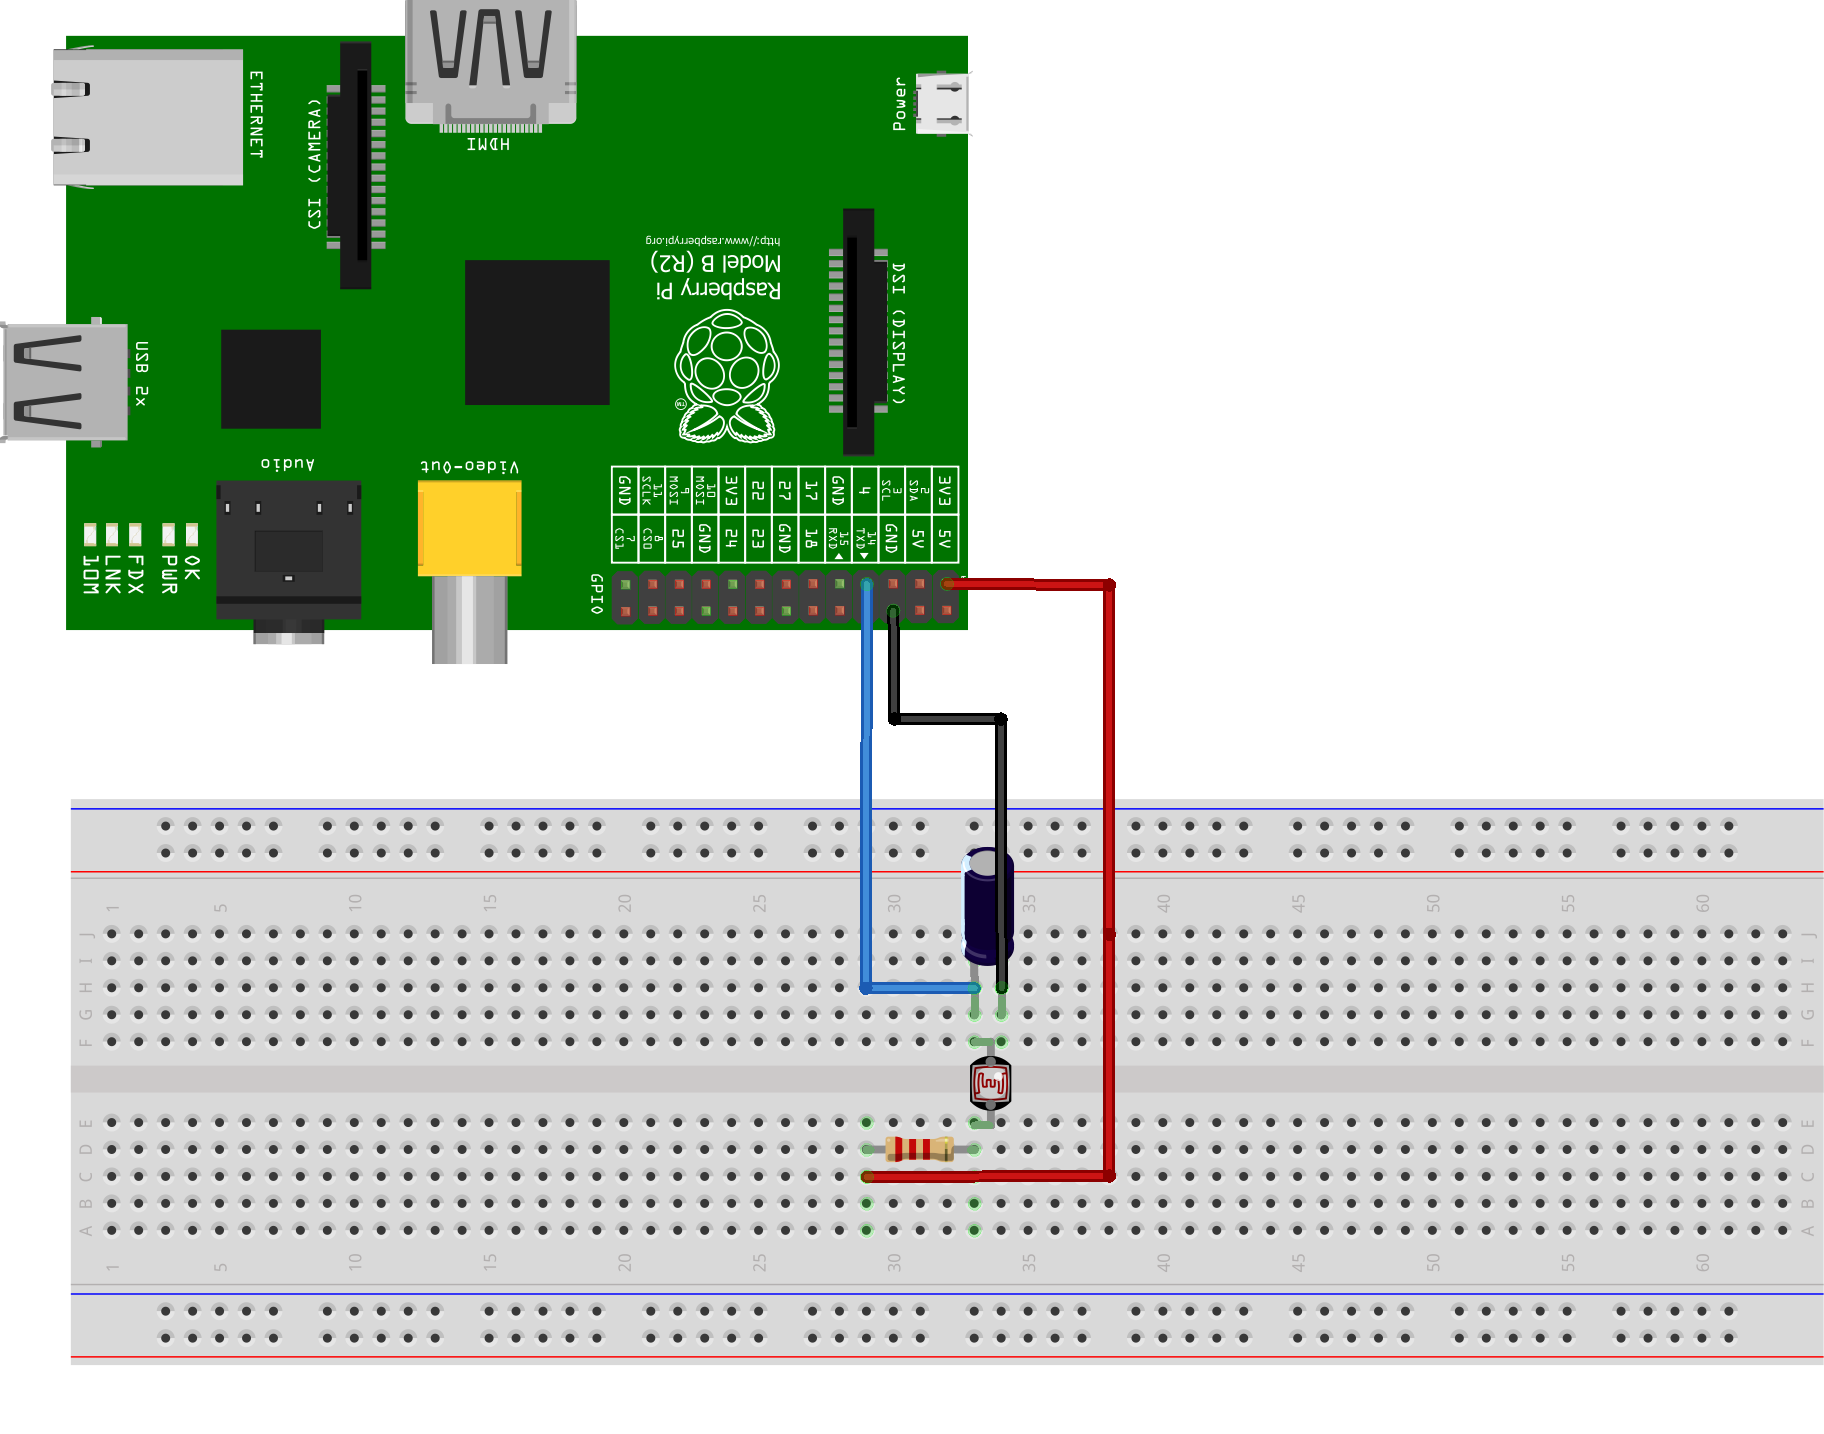
\includegraphics[scale=0.15]{./img/sensor_bb.png}
\caption{Sensor}
\end{figure}
% \begin{minipage}{\linewidth}
\\\noindent
W układzie o którym mowa w tym rozdziale rezystor $2.2k \Omega$ działa jako zabezpieczenie przed zbyt dużym napięciem skierowanym na port GPIO. Podłączony jest do fotorezystora, którego rezystancja jest niska kiedy świeci na niego wiązka lasera. Kondensator $1\mu F$ jest ładowany a kiedy przekroczy wartość graniczną wynoszącą około 2V pin GPIO rejestruje wartość HIGH. Działanie to jest wykorzystane w kodzie aplikacji gdzie mierzony jest czas potrzebny na naładowanie kondensatora. Kiedy czas jest krótki znaczy to że na fotorezystor pada wiązka lasera, kiedy się zwiększy znaczy to że laser został przecięty tj. zawodnik przejechał przez start lub metę.
\newpage
\subsection{Implementacja}
Ninejszy rozdział zostanie poświęcony implementacji. Składa się on z dwóch podrozdziałów: Aplikacja, który opisuję budowę aplikacji startowej oraz rozdziału Worker opisującego worker rejestrujący przejechanie mety.
\subsubsection{Aplikacja}
Tak jak była o tym mowa we wstępie do ninejszej pracy aplikację startową można podzielić na dwa osobne komponenty. Jeden stanowi aplikacja napisana we frameworku Sinatra, która udostępnia API dla aplikacji front-end do komunikacji z bazą danych. Ona także serwuje skompilowane zasoby. W momencie uruchomienia aplikacji jest też tworzony nowy wątek, którego zadaniem jest zarejestrowanie startu. 
	Aplikacja front-end natomiast dostarcza interfejs dostępny przez przeglądarke internetową służący do interakcji z back-endem.
\begin{listing}[H]
\inputminted[linenos=true]{ruby}{./src/thread.rb}
\caption{Wątek rejestrujący przejechanie mety}
$\label{thread}$
\end{listing}
%\end{minipage}
\newpage
\noindent
Wykorzystana tutaj klasa Injector, ma za zadanie budowanie obiektów używających dependency injection w raz z wszelkimi zależnościami przy pomocy gemu Dependor. 


% W swoim konstuktorze oczekuje obiektów Sinatra dlatego tutaj inicjalizowana jest pustym objektem OpenStruct. OpenStruct odpowiada na dowolne metody oraz zwraca \emph{nil} jeśli nazwa metody wywołanej na rzecz tego obiektu nie zawiera się w haszu, który został użyty do inicjalizacji. 
Obiekt klasy Injector jest 	przekazywany w bloku, gdzie póżniej dostarcza obiektów takich jak \emph{capacitor}, którego klasa jest zdefiniowana w pliku \newline \emph{app/services/components/capacitor.rb}. 

W klasie Injector są definiowane moduły które mają być przeszukane w poszukiwaniu klas, które maja być wstrzykiwane co przedstawia listing \ref{injector}. Nazwy przyjmowane w argumentach metody \emph{takes} oraz nazwy metod wywołanych na obiekcie Injector odpowiadają nazwom plików wstrszykiwanych klas. Warunkiem tego jest odpowiednie nazewnictwo klas i plików zgodnie z konwencjami przyjętymi w programowaniu Ruby.

W Ruby przyjęło się nazywanie nazw klas i modułów z dużej litery \mbox{CamelCase} a pliki zawierające te klasy powinny mieć taką samą nazwę jak klasa tylko zapisaną w snake\_case z rozszerzeniem *.rb.
\begin{listing}[H]
\inputminted[linenos=true]{ruby}{./src/injector.rb}
\caption{Klasa injector odpowiedzialna za tworzenie obiektów z wykorzystaniem DI}
$\label{injector}$
\end{listing}
\noindent
Powyższy listing przedstawia jedynie fragment klasy Injector ponieważ jest zbyt długa aby ją całą zamieścić. 

Pozostałe metody klasy zawierają jedynie obiekty lub nazwy stałych, które są wstrzykiwane. W konstruktorze klasy Injector jest też inicjalizowane GPIO (General Purpose Input Output).

Obsługę GPIO zapewnia WiringPi-Ruby|wrapper Ruby popularnej biblioteki C WiringPi. W klasie Injector defniuje go metoda pokazana na listingu \ref{io}

\begin{listing}[H]
\inputminted[linenos=true]{ruby}{./src/io.rb}
\caption{WiringPi}
$\label{io}$
\end{listing}
\noindent
Metoda \emph{io} jest wstrzykiwana do klasy RaspberryPi::Gpio, która jest odpowiedzialna za ustawienie odpowiedniego kierunku pinu (INPUT|OUTPUT) oraz napisanie lub pobranie z niego.

\begin{listing}[H]
\inputminted[linenos=true]{ruby}{./src/gpio.rb}
\caption{app/services/rasperry\_pi/gpio.rb}
$\label{gpio}$
\end{listing}
\noindent
Ta sama klasa \ref{gpio} użyta jest w workerze. Jest to jedna z zalet obiektowości a w szczególności dependency injection ponieważ klasa nie ma żadnych bezpośrenich zależności i może być łatwo przeniesiona do innej aplikacji. Klasa \emph{RaspberryPi::Gpio} jest w tej aplikacji użyta jedynie w klasie \emph{Components::Capacitor} \ref{capacitor}.
\begin{listing}[H]
\inputminted[linenos=true]{ruby}{./src/capacitor.rb}
\caption{app/services/components/capacitor.rb}
$\label{capacitor}$
\end{listing}
\noindent
Zadaniem tej klasy jest napisanie wartości LOW na pin w celu rozładowania ładunku na kondensatorze. 

 
Dzieje się to na początku pętli \emph{while} w wątku z listingu \ref{thread}. Następnie w tej samej pętli \emph{śpimy} przez 1ms oraz odczyt ustawiany jest na zero. W kolejnej pętli \emph{while} pin GPIO jest ustawiany na wejście, pobierana jest z niego wartość a kiedy kondensator przekroczy wartość graniczną jest zwracany jest odczyt inkrementowany w tej pętli. 
 
Jeśli jego wartość przekroczy zadany czas potrzebny na naładowanie kondensatora (tutaj próg aktywacji) w Memcached ustawiany jest dokładny czas tego zdarzenia pod kluczem \emph{start\_time}. Odpowiedzialna jest za to klasa CachingService przedstawiona na listingu \ref{caching}.
\newpage
\begin{listing}[H]
\inputminted[linenos=true]{ruby}{./src/cachingservice.rb}
\caption{app/services/caching\_service.rb}
$\label{caching}$
\end{listing}
\noindent
Klasa w konstruktorze jako argument przyjume obiekt klasy \mbox{MemcacheConnection} pokazanej na listingu \ref{mcon}. Metody tej klasy \emph{get} oraz \emph{set} mają oczywiste działanie zatem zostaną pominięte. Warto jednak zwrócić uwagę na metodę fetch która próbuje pobrać wartość z cache a kiedy nic nie znajduje się pod przekazanym kluczem wywołuje metodę \emph{set} ustawiającą klucz wartością zwracaną przez przekazany blok. Przykładowe użycie tej metody przedstawiono poniżej.
\begin{listing}
\inputminted[linenos=true]{ruby}{./src/fetch.rb}
\caption{Przykład wykorzystania metody fetch.}
\end{listing}
\newpage
\noindent
Klasa Connections::MemcaheConnection przyjmuje tutaj w metodzie takes symbol \emph{:dalli\_client}, który jest nazwą nazwą metody zawartej w klasie Injector zwracającą klasę \emph{Dalli::Client}.
\begin{listing}
\inputminted[linenos=true]{ruby}{./src/memcache.rb}
\caption{app/services/connections/memcache.rb}
$\label{mcon}$
\end{listing}
\paragraph{API} ~\\
API dla aplikacji Backbone (interfejsu) zostało napisane we frameworku Sinatra. Framework ten został  zaprojektowany do pisania niewielkich, lekkich aplikacji web i został wybrany ponieważ autor uznał że Ruby on Rails (najpopularnieszy framework Ruby) jest zbyt rozbudowany i uruchomienie aplikacji RoR na RaspberryPi mogło by zużyć zbyt wiele zasobów urządzenia. Sama aplikacja Sinatra uruchamiana jest na porcie 9292. Z tego powodu znajuję się za proxy | serwerem Nginx, który przekierowuje zapytania przychodzące na port 80 na aplikację.

Typowo aplikacjia Sinatra składa się z jednej klasy. W celu wprowadzenia porządku autor zdecydował się ją rozbić na miejsze pliki. Jako pierwszy załączany jest plik \emph{application.rb}, który min. zawiera deklarację modułów, konfigurację Sprockets oraz konfigurację Warden, która zostanie omówiona w rozdziale \ref{warden}. Na końcu załączane są pozostałe piliki zawierające poszczególne end-pointy, które monkey patchują klasę. Znajdują się w folderze \emph{app/routes} i zostaną przedstawione poniżej przy pomocy zapytań curl i odpowiedzi. W celu autentykacji najpierw wykonane jest rządanie POST z login oraz hasłem. Potem możemy autentykować się przy pomocy cookie. 
\begin{listing}
\inputminted{sh}{./src/curl_auth}
\end{listing}
\newpage	
W przypadku udanego logowania serwer odpowiada JSONem
\begin{listing}
\inputminted{json}{./src/curl_auth_response}
\end{listing} 
\subparagraph{Contestants} ~\\
W pliku \emph{app/routes/contestants.rb} zawarte są 2 endpointy: \newline\mbox{GET \emph{/contestants/:id}} zwracający zawodnika o podanym id oraz,\newline POST \emph{/contestants} służący do tworzenia nowych zawodników.
\begin{listing}
\inputminted{sh}{./src/curl_get_contestant}
\caption{GET \emph{/contestants/:id}}
\end{listing}
\begin{listing}
\inputminted{json}{./src/curl_get_contestant_response}
\caption{Odpowiedź zwracana przez GET \emph{/contestants/1}}
\end{listing}

Przy tworzeniu zawodnika jest zwracany jedynie kod odpowiedzi HTTP. Jeśli dane są poprawne i zawodnik zostanie zapisany do bazy zwracany jest kod 200 (OK) w przeciwnym wypadku zwracany jest kod błędu 422 (Unprocessable Entity).
\newpage
%\begin{minipage}{\textwidth}
\begin{listing}
\inputminted{sh}{./src/curl_post_contestants}
\caption{POST \emph{/contestants}}
\end{listing}
Do metody get '/contestants/:id' przekazywane są w bloku dwie zmienne: contestant\_presenter oraz cotestant\_repository. contestant\_presenter jest obiektem klasy Presenters::ContestantPresenter, której zadaniem jest prezentacja kolekcji zawodników w formatach JSON, CSV, XML oraz jako Hasz.

Użyta tutaj metoda \emph{as\_json} mapuje przekazaną kolekcję na tablicę haszy oraz wywołuje na zwracanej wartości metodę \emph{to\_json} co przedstawia listing \ref{as_json}.
\begin{listing}
\inputminted{ruby}{./src/contestants_as_json.rb}
\caption{\emph{app/services/presenters/contestant\_presenter.rb}}
$\label{as_json}$
\end{listing}


Przekazywana także w bloku metody \emph{post} zmienna contestant\_repository jest obiektem klasy \emph{Repositories::ContestantRepository} mającej za zadanie budowę, zapis oraz pobieranie z bazy zawodników \ref{contestant_repository}. W konstruktorze przyjmuję między innymi model zawodnika. %\newline\emph{app/models/contestant.rb}.

W bloku metody post przekazywane są też zmienne hash i json\_parser metody klasy \emph{Injector} zwracającej stałą JSON, która jest potem użyta do sparsowania ciała żądania HTTP. hash jest obiektem klasy Hash modułu \emph{Skirace}. Klasa ta dziedziczy po Haszu i ma na celu dodanie pomocniczych metod znanych z Rails takich jak użyta tutaj \emph{with\_indifferent\_access} pozwalająca na odwołanie się do klucza haszu przy pomocy stringa lub symbolu. 

Takie podejście zostało wybrane ponieważ autor uważa że monkey patchowanie klas należących do \emph{Ruby core} jest czymś czego nie powinno się robić. 
\begin{listing}
\inputminted{ruby}{../app/services/repositories/contestant_repository.rb}
\caption{\emph{app/services/repositories/contestant\_repository.rb}}
$\label{contestant_repository}$
\end{listing}
%\newpage
\clearpage
\subparagraph{Contests} ~\\
W pliku \emph{app/routes/contests.rb} znajdują się następujące endpointy:
\\
GET \emph{/contests}
\\
\noindent
Zwraca wszystkie zawody z bazy.
\begin{listing}
\inputminted{ruby}{./src/get_contests.rb}
\caption{\emph{app/routes/contests.rb}}
$\label{contests}$
\end{listing}
\begin{listing}
\inputminted{ruby}{./src/curl_contests}
\caption{GET \emph{/contests}}
\end{listing}
\begin{listing}
\inputminted{ruby}{./src/curl_contests_resp}
\caption{JSON response}
\end{listing}
Zmienna contest\_presenter przekazana w bloku jest obiektem klasy \emph{Presenters::ContestPresenter} zawieającej jedynie metodę \emph{as\_json} działającą analogicznie do metody o tej samej nazwie klasy \emph{Presenters::ContestantPresenter} przedstawionej wcześniej.

\indent contest\_repository jest tutaj obiektem klasy \emph{Repositories::ContestRepository}. Metoda all najpierw sprawdza czy w bazie znajdują się zawody metodą \emph{any?} Jeśli w bazie danych istnieją zawody są one zwracane w przeciwnym wypadku wywoływana jest prywatna metoda \emph{create\_default} (\ref{contest_create_default}).
\begin{listing}
\inputminted{ruby}{./src/contest_create_default.rb}
\caption{\emph{app/services/repositories/contest\_repository.rb}}
$\label{contest_create_default}$
\end{listing}
\newpage
\noindent
GET \emph{/contests/public}
\\
\noindent
Jeśli publicznie udostępnianie zawodów jest włączone zwrócony zostanie JSON zawierający id i nazwę zawodów oraz listę zawodników \ref{public_contest_on} w przeciwnym wypadku zwrócony zostanie JSON z odpowiedzią \emph{no-public-contests} oraz statusem HTTP 404 (Not Found) \ref{public_contest_off}.
\begin{listing}
\inputminted{ruby}{./src/get_contest_public.rb}
\caption{\emph{app/routes/contests.rb}}
$\label{get_contest_public}$
\end{listing}
\begin{listing}
\inputminted{ruby}{./src/curl_public_contest}
\caption{GET \emph{/contests/public}}
\end{listing}
\newpage
%\begin{minipage}[c]{\textwidth}
\begin{listing}
\inputminted{json}{./src/curl_public_contest_on}
\caption{Publiczne udostępnianie zawodów włączone}
$\label{public_contest_on}$
\end{listing}
\begin{listing}
\inputminted{json}{./src/curl_public_contest_off}
\caption{Publiczne udostępnianie zawodów wyłączone}
$\label{public_contest_off}$
\end{listing}
\noindent
GET \emph{/contests/:id/contestants}
\\
\noindent
Zwraca listę zawodników dla zawodów o przekazanym id.
\begin{listing}
\inputminted{ruby}{./src/contest_contestants.rb}
\caption{\emph{app/routes/contests.rb}}
\end{listing}
\begin{listing}[H]
\inputminted{ruby}{./src/curl_contest_contestants}
\caption{GET \emph{/contests/1/contestants}}
\end{listing}
% \\
\begin{listing}[H]
\inputminted{json}{./src/curl_contest_contestants_response}
\caption{Odpowiedź JSON}
\end{listing}
%\end{minipage}
% \\
% \newpage
% \noindent
POST \emph{/contests}
\\
\noindent
Tworzy nowe zawody.
\begin{listing}[H]
\inputminted{ruby}{./src/contest_curl}
\caption{POST \emph{/contests}}
\end{listing}
\noindent
Ten endpoint odpowiada jedynie kodem statusu HTTP 200 (OK) jeśli utworzenie nowych zawodów się powiedzie oraz 422 (Unprocessable entity) w przeciwnym wypadku.
\newline
\newline
\noindent
PUT \emph{/contests/current}
\\
\noindent
Ma na celu ustawianie aktualnie wybranych zawodów w Memcached. Podobnie jak powyższy endpoint zwraca jedynie w odpowiedzi kod statusu.
\begin{listing}[H]
\inputminted{ruby}{./src/curl_current_contest}
\caption{PUT \emph{/contests/current}}
\end{listing}
% TODO: MOAR ENDPOINTS
%\begin{listing}
%\inputminted{ruby}{../app/routes/contestants.rb}
%\caption{\emph{app/routes/contestants.rb}}
%$\label{contestants}$
%\end{listing}
%\end{minipage}
\paragraph{Warden}\label{warden} ~\\
W celu autentykacji użytkowników aplikacji został wykorzystany gem Warden będący oprogramowaniem pośredniczącym (\emph{eng. middleware}) dla aplikacji Rack. Warden wstrzykuje \emph{leniwy obiekt} (który jest inicjalizowany tylko wtedy kiedy zajdzie na niego zapotrzebowanie) do env['warden']. Pozwala on np. na sprawdzenie czy użytkownik jest zalogowany env['warden'].authenticated? Warden pozwala na definiowanie strategii autentykowania użytkowników. Każda ze zdefiniowanych strategii będzie próbowała zautentykować użytkownika aplikacji aż któraś z nich się powiedzie. Strategie autentykacji, która została użyta w tym projekcie przedstawia listing \ref{strategy}.

\begin{listing}[H]
\inputminted[linenos=true]{ruby}{./src/warden_strategy.rb}
\caption{Strategia autentykacji}
$\label{strategy}$
\end{listing}
\newpage
\paragraph{Front-end} ~\\
Inerface apllikacji, tak jak była to tym mowa we wstępie, został napisany przy pomocy Backbone.js. Aplikacja frontend jest inicjalizowana ostatnią linią listingu \ref{aplication-js}. Obiekty aplikacji oraz funkcja inicjalizująca ją są zawarte w pliku \emph{app.coffee} przedstawionym na listingu \ref{app-coffee}. 
\begin{listing}[H]
\inputminted{js}{./src/app.coffee}
\caption{app/assets/javascripts/app.coffee}
$\label{app-coffee}$
\end{listing}

\subsubsection{Worker}
Worker o którym była mowa we wstępie do niniejszej pracy rejestruje przejechanie linii mety. Został on napisany w całości w języku Ruby jako \emph{gem} - program managera paczek RubyGems. Po zainstalowaniu w systemie dostarcza on komendy \emph{skirace-worker}, która go uruchamia.


Po uruchominiu startuje pętlę pobierającą wartość z czujnika a w momencie przejechania mety wysyła rządanie POST do aplikacji startowej oraz w odpowiedzi otrzymuje imię, nazwisko i czas końcowy zawodnika oraz wyświetla je na wyświetlaczu LCD zgodnym ze standardem HD44780. Strukturę oraz informacje o gemie definiuje plik \emph{skirace-worker.gemspec}, który zawiera klasę ze specyfikacją.

Plikiem wykonywalnym gemu jest skrypt Ruby, który załącza plik \emph{lib/skirace\_worker.rb} zawierający definicje modułów workera. Dadaje on też kolejne pliki oraz klasy a następnie uruchamia worker (\ref{binary}). 

\begin{listing}
\inputminted[linenos=true]{ruby}{./src/binary}
\caption{bin/skirace-worker}
$\label{binary}$
\end{listing}



\newpage
\subsection{Obudowa ochronna}
Obudowa urządzenia została wykonana ze skrzynek izolacyjnych D25 montowancyh na rurach kanalizacyjncyh PP 50/1000 mm przy pomocy opasek zaciskowych. W skrzynkach znajduje się RaspberryPI przykręcone do wygiętego fragmentu opakowania na płyty CD na warstwie ochronnej wycinku karimaty, koszyczek na 6 baterii AA dostarczający zasilanie oraz układ UBEC - przetwornica impulsowa - redukująca napięcie z baterri do 5V 3A dla bramki startowej, oraz 5V 5A dla bramki końcowej.
\newpage
\section{Licencje Gemów}
\subsection{Wykaz gemów}
\begin{itemize}
\item \textbf{execjs}  \\
Autorzy: Sam Stephenson, Josh Peek \\
Licencja: MIT
\item \textbf{haml} MIT \\
Autorzy: Hampton Catlin, Nathan Weizenbaum \\
Licencja: MIT
\item \textbf{haml\_coffee\_assets} \\
Autor: Michael Kessler \\
Licencja: MIT
\item \textbf{uglifier} \\
Autor: Ville Lautanala \\
Licencja: MIT
\item \textbf{sinatra} \\
Autorzy: Blake Mizerany, Konstantin Haase \\
Licencja: MIT 
\item \textbf{sequel} \\
Autorzy: Sharon Rosner, Jeremy Evans \\
Licencja: MIT
\item \textbf{sprockets} \\
Autorzy: Sam Stephenson, Josua Peek \\
Licencja: MIT
\item \textbf{sprockets-helpers} \\ 
Autor: Perer Browne \\
Licencja: MIT
\item \textbf{dependor-sinatra} \\ 
Autor: Adam Pohorecki \\
Licencja: MIT
\item \textbf{therubyracer} \\ 
Autor: Charles Lowell \\
Licencja: MIT
\item \textbf{wiringpi} GNU LGPLv3
\item \textbf{thin} \\ 
Autor: Marc-Andre Cournoyer \\
Licencja: Ruby
\item \textbf{sqlite3} \\ 
Autorzy: Jamis Bluck, Luis Lavena, Aron Patterson \\
Licencja: BSD-3
\item \textbf{sass} \\
Autorzy: Nathan Weizenbaum, Chris Eppstein, Hampton Catlin \\
Licancja: MIT
\item \textbf{binding\_of\_caller} \\ 
Autor: John Mair \\
Licencja: MIT
\item \textbf{pry} \\
Autorzy: John Mair, Conrad Irwin, Ryan Fitzgerald \\
Licencja: MIT
\item \textbf{warden} \\ 
Autor: Daniel Neighman \\
Licencja: MIT
\item \textbf{bcrypt-ruby} \\ 
Autor: Coda Hale \\
Licencja: MIT
\item \textbf{memcache-client} \\
Autorzy: Eric Hodel, Robert Cottler, Mike Perham \\
Licencja:  BSD-3
\item \textbf{dalli} \\ 
Autor: Mike Perham \\
Licencja: MIT
\item \textbf{nokogiri} \\ 
Autorzy: Aaron Patterson, Mike Dalessio, Yoko Harada, Tim Eliott, Akinori MUSHA  \\
Licencja: MIT
\end{itemize}
\newpage

\subsection{Treści licencji}
\subsubsection{MIT}
Permission is hereby granted, free of charge, to any person obtaining
a copy of this software and associated documentation files (the
"Software"), to deal in the Software without restriction, including
without limitation the rights to use, copy, modify, merge, publish,
distribute, sublicense, and/or sell copies of the Software, and to
permit persons to whom the Software is furnished to do so, subject to
the following conditions:

The above copyright notice and this permission notice shall be
included in all copies or substantial portions of the Software.

THE SOFTWARE IS PROVIDED "AS IS", WITHOUT WARRANTY OF ANY KIND,
EXPRESS OR IMPLIED, INCLUDING BUT NOT LIMITED TO THE WARRANTIES OF
MERCHANTABILITY, FITNESS FOR A PARTICULAR PURPOSE AND
NONINFRINGEMENT. IN NO EVENT SHALL THE AUTHORS OR COPYRIGHT HOLDERS BE
LIABLE FOR ANY CLAIM, DAMAGES OR OTHER LIABILITY, WHETHER IN AN ACTION
OF CONTRACT, TORT OR OTHERWISE, ARISING FROM, OUT OF OR IN CONNECTION
WITH THE SOFTWARE OR THE USE OR OTHER DEALINGS IN THE SOFTWARE.
\newpage
\subsubsection{LGPLv3}
Everyone is permitted to copy and distribute verbatim copies of this license document, but changing it is not allowed.

This version of the GNU Lesser General Public License incorporates the terms and conditions of version 3 of the GNU General Public License, supplemented by the additional permissions listed below.

\begin{enumerate}
\addtocounter{enumi}{-1}  % start at 0

\item Additional Definitions.

  As used herein, ``this License'' refers to version 3 of the GNU Lesser
General Public License, and the ``GNU GPL'' refers to version 3 of the GNU
General Public License.

  ``The Library'' refers to a covered work governed by this License,
other than an Application or a Combined Work as defined below.

  An ``Application'' is any work that makes use of an interface provided
by the Library, but which is not otherwise based on the Library.
Defining a subclass of a class defined by the Library is deemed a mode
of using an interface provided by the Library.

  A ``Combined Work'' is a work produced by combining or linking an
Application with the Library.  The particular version of the Library
with which the Combined Work was made is also called the ``Linked
Version''.

  The ``Minimal Corresponding Source'' for a Combined Work means the
Corresponding Source for the Combined Work, excluding any source code
for portions of the Combined Work that, considered in isolation, are
based on the Application, and not on the Linked Version.

  The ``Corresponding Application Code'' for a Combined Work means the
object code and/or source code for the Application, including any data
and utility programs needed for reproducing the Combined Work from the
Application, but excluding the System Libraries of the Combined Work.

\item Exception to Section 3 of the GNU GPL.

  You may convey a covered work under sections 3 and 4 of this License
without being bound by section 3 of the GNU GPL.

\item Conveying Modified Versions.

  If you modify a copy of the Library, and, in your modifications, a
facility refers to a function or data to be supplied by an Application
that uses the facility (other than as an argument passed when the
facility is invoked), then you may convey a copy of the modified
version:

   \begin{enumerate}
   \item under this License, provided that you make a good faith effort to
   ensure that, in the event an Application does not supply the
   function or data, the facility still operates, and performs
   whatever part of its purpose remains meaningful, or

   \item under the GNU GPL, with none of the additional permissions of
   this License applicable to that copy.
   \end{enumerate}

\item Object Code Incorporating Material from Library Header Files.

  The object code form of an Application may incorporate material from
a header file that is part of the Library.  You may convey such object
code under terms of your choice, provided that, if the incorporated
material is not limited to numerical parameters, data structure
layouts and accessors, or small macros, inline functions and templates
(ten or fewer lines in length), you do both of the following:

   \begin{enumerate}
   \item Give prominent notice with each copy of the object code that the
   Library is used in it and that the Library and its use are
   covered by this License.

   \item Accompany the object code with a copy of the GNU GPL and this license
   document.
   \end{enumerate}

\item Combined Works.

  You may convey a Combined Work under terms of your choice that,
taken together, effectively do not restrict modification of the
portions of the Library contained in the Combined Work and reverse
engineering for debugging such modifications, if you also do each of
the following:

   \begin{enumerate}
   \item Give prominent notice with each copy of the Combined Work that
   the Library is used in it and that the Library and its use are
   covered by this License.

   \item Accompany the Combined Work with a copy of the GNU GPL and this license
   document.

   \item For a Combined Work that displays copyright notices during
   execution, include the copyright notice for the Library among
   these notices, as well as a reference directing the user to the
   copies of the GNU GPL and this license document.

   \item Do one of the following:

       \begin{enumerate}
       \addtocounter{enumiii}{-1}  % start at 0
       \item Convey the Minimal Corresponding Source under the terms of this
       License, and the Corresponding Application Code in a form
       suitable for, and under terms that permit, the user to
       recombine or relink the Application with a modified version of
       the Linked Version to produce a modified Combined Work, in the
       manner specified by section 6 of the GNU GPL for conveying
       Corresponding Source.

       \item Use a suitable shared library mechanism for linking with the
       Library.  A suitable mechanism is one that (a) uses at run time
       a copy of the Library already present on the user's computer
       system, and (b) will operate properly with a modified version
       of the Library that is interface-compatible with the Linked
       Version. 
       \end{enumerate}

   \item Provide Installation Information, but only if you would otherwise
   be required to provide such information under section 6 of the
   GNU GPL, and only to the extent that such information is
   necessary to install and execute a modified version of the
   Combined Work produced by recombining or relinking the
   Application with a modified version of the Linked Version. (If
   you use option 4d0, the Installation Information must accompany
   the Minimal Corresponding Source and Corresponding Application
   Code. If you use option 4d1, you must provide the Installation
   Information in the manner specified by section 6 of the GNU GPL
   for conveying Corresponding Source.)
   \end{enumerate}

\item Combined Libraries.

  You may place library facilities that are a work based on the
Library side by side in a single library together with other library
facilities that are not Applications and are not covered by this
License, and convey such a combined library under terms of your
choice, if you do both of the following:

   \begin{enumerate}
   \item Accompany the combined library with a copy of the same work based
   on the Library, uncombined with any other library facilities,
   conveyed under the terms of this License.

   \item Give prominent notice with the combined library that part of it
   is a work based on the Library, and explaining where to find the
   accompanying uncombined form of the same work.
   \end{enumerate}

\item Revised Versions of the GNU Lesser General Public License.

  The Free Software Foundation may publish revised and/or new versions
of the GNU Lesser General Public License from time to time. Such new
versions will be similar in spirit to the present version, but may
differ in detail to address new problems or concerns.

  Each version is given a distinguishing version number. If the
Library as you received it specifies that a certain numbered version
of the GNU Lesser General Public License ``or any later version''
applies to it, you have the option of following the terms and
conditions either of that published version or of any later version
published by the Free Software Foundation. If the Library as you
received it does not specify a version number of the GNU Lesser
General Public License, you may choose any version of the GNU Lesser
General Public License ever published by the Free Software Foundation.

  If the Library as you received it specifies that a proxy can decide
whether future versions of the GNU Lesser General Public License shall
apply, that proxy's public statement of acceptance of any version is
permanent authorization for you to choose that version for the
Library.

\end{enumerate}
\subsubsection{Ruby}
Ruby is copyrighted free software by Yukihiro Matsumoto matz@netlab.jp.
You can redistribute it and/or modify it under either the terms of the
2-clause BSDL (see the file BSDL), or the conditions below:
\begin{enumerate}
\item  You may make and give away verbatim copies of the source form of the
     software without restriction, provided that you duplicate all of the
     original copyright notices and associated disclaimers.
\item You may modify your copy of the software in any way, provided that
     you do at least ONE of the following:
     \begin{enumerate}
     	\item  place your modifications in the Public Domain or otherwise
          make them Freely Available, such as by posting said
	  modifications to Usenet or an equivalent medium, or by allowing
	  the author to include your modifications in the software.
	  	\item use the modified software only within your corporation or
          organization.
        \item give non-standard binaries non-standard names, with
          instructions on where to get the original software distribution.
        \item make other distribution arrangements with the author.
     \end{enumerate}
\item You may distribute the software in object code or binary form,
     provided that you do at least ONE of the following:
     \begin{enumerate}
     	\item distribute the binaries and library files of the software,
	  together with instructions (in the manual page or equivalent)
	  on where to get the original distribution.
	  	\item accompany the distribution with the machine-readable source of
	  the software.
	  	\item give non-standard binaries non-standard names, with
          instructions on where to get the original software distribution.
        \item make other distribution arrangements with the author.
     \end{enumerate}
\item You may modify and include the part of the software into any other
     software (possibly commercial).  But some files in the distribution
     are not written by the author, so that they are not under these terms.

     For the list of those files and their copying conditions, see the
     file LEGAL.
\item The scripts and library files supplied as input to or produced as 
     output from the software do not automatically fall under the
     copyright of the software, but belong to whomever generated them, 
     and may be sold commercially, and may be aggregated with this
     software.
\item THIS SOFTWARE IS PROVIDED "AS IS" AND WITHOUT ANY EXPRESS OR
     IMPLIED WARRANTIES, INCLUDING, WITHOUT LIMITATION, THE IMPLIED
     WARRANTIES OF MERCHANTABILITY AND FITNESS FOR A PARTICULAR
     PURPOSE.
\end{enumerate}
\subsubsection{BSD-3}
Redistribution and use in source and binary forms, with or without modification, are permitted provided that the following conditions are met:
\begin{enumerate}

\item Redistributions of source code must retain the above copyright notice, this list of conditions and the following disclaimer.

\item Redistributions in binary form must reproduce the above copyright notice, this list of conditions and the following disclaimer in the documentation and/or other materials provided with the distribution.

\item Neither the name of the copyright holder nor the names of its contributors may be used to endorse or promote products derived from this software without specific prior written permission.

\end{enumerate}
THIS SOFTWARE IS PROVIDED BY THE COPYRIGHT HOLDERS AND CONTRIBUTORS "AS IS" AND ANY EXPRESS OR IMPLIED WARRANTIES, INCLUDING, BUT NOT LIMITED TO, THE IMPLIED WARRANTIES OF MERCHANTABILITY AND FITNESS FOR A PARTICULAR PURPOSE ARE DISCLAIMED. IN NO EVENT SHALL THE COPYRIGHT HOLDER OR CONTRIBUTORS BE LIABLE FOR ANY DIRECT, INDIRECT, INCIDENTAL, SPECIAL, EXEMPLARY, OR CONSEQUENTIAL DAMAGES (INCLUDING, BUT NOT LIMITED TO, PROCUREMENT OF SUBSTITUTE GOODS OR SERVICES; LOSS OF USE, DATA, OR PROFITS; OR BUSINESS INTERRUPTION) HOWEVER CAUSED AND ON ANY THEORY OF LIABILITY, WHETHER IN CONTRACT, STRICT LIABILITY, OR TORT (INCLUDING NEGLIGENCE OR OTHERWISE) ARISING IN ANY WAY OUT OF THE USE OF THIS SOFTWARE, EVEN IF ADVISED OF THE POSSIBILITY OF SUCH DAMAGE.
\newpage
\section{Summary}
\end{document}